\documentclass[11pt,a4paper]{report}

\usepackage[utf8]{inputenc}
\usepackage[T1]{fontenc}

\usepackage{amsmath}
\pagestyle{empty}

\usepackage{graphicx} % Include figure files
\usepackage{amstext,amsbsy,amssymb}
%\usepackage{times} 

%% Numbered problems
\newcounter{excount}[chapter]
\newenvironment{exercise}[1][]{\addtocounter{excount}{1} \noindent {\bf Problem
    \arabic{excount} \ \ #1}\hspace{2mm}}{\vspace{4mm}}


\title{FYS3120 Classical Mechanics and Electrodynamics\\ 
\vspace{15mm}Problem set 4}


%%%%%%%
\begin{document}
%%%%%%%
\author{Johan Nereng}
\maketitle


%%%%%%%%
\begin{exercise}
The figure shows a rod of length $b$ and mass $m$, with the mass evenly distributed along the rod.
One endpoint of the rod is constrained to move along a horisontal line and the other endpoint along a vertical line. The two lines are in the same plane. There is no friction and the acceleration due to gravity is $g$. The set-up is illustrated in Fig.~\ref{fig:con_rod}.

%%%%%%%%%%
\begin{figure}[h]
\begin{center}
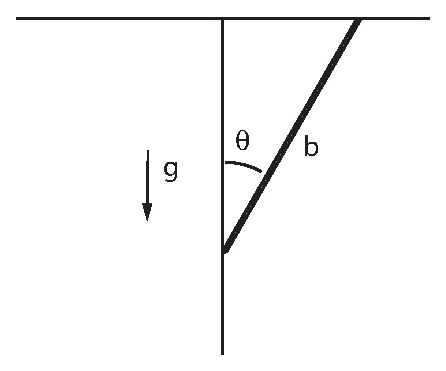
\includegraphics[width=5cm]{ConstrainedRod.eps}
\end{center}
\caption{Constrained rod.}
\label{fig:con_rod}
\end{figure}
%%%%%%%%%% 

\begin{itemize}
\item[\bf a)] Find the Lagrangian $L$ with the angle $\theta$ as coordinate, and show that Lagrange's equation gives
\begin{equation}
\ddot\theta+{3g\over {2b}}\sin\theta=0.
\end{equation}
{\it Hint:} For the moment of inertia of the rod, see Problem 2 in Set 2.
%%%%%%%%%%%%%%%%%%%%%%%%%% 

\item $K=\frac{1}{2}I\dot{\theta}^2=\frac{b}{2}\frac{1}{3}mb^2\dot{\theta}^2$, $V=-mg\frac{b}{2}cos \theta$
\item $L=K-V=\frac{1}{2}\frac{1}{3}mb^2\dot{\theta}^2+mg\frac{b}{2}cos \theta$
\item $\frac{dL}{dt}(\frac{\partial L}{\partial \dot{\theta}})-\frac{\partial L}{\partial \theta}=\frac{1}{3}mb^2\ddot{\theta}+mg\frac{b}{2}sin \theta=\ddot{\theta}+\frac{3g}{2b}sin\theta=0$




%%%%%%%%%%%%%%
\item[\bf b)] What is the stable equilibrium position of the rod? Find the period $T_0$ for small oscillations about equilibrium.
\item The stable equilibrium position is $\theta=0$
\item Small angle approximation  yields:
$\ddot{\theta}+\frac{3g}{2b}\theta=0 \implies \theta(t)=\theta_0 cos (\omega t)$, where $\omega=\sqrt{\frac{3g}{2b}}$, thus $T_0=\frac{2\pi}{\omega}=2\pi\sqrt{\frac{2b}{3g}}$

%%%%%%%%%%%%%%%%%%%%%%%%%% 
\item[\bf c)] Since $L$ has no explicit time dependence, there is a corresponding constant of motion. What is the expression for this constant and what is the physical interpretation? Comment on how the expression is related to the equation of motion.

\item constant of motion $p_1=\frac{\partial L}{\partial \dot{\theta}}=\frac{1}{3}mb^2\dot{\theta}=I\dot{\theta}$, or the angular momentum, which is conserved. This means that a change in $\dot{\theta}$ does not change the equation of motion.

%%%%%%%%%%%%%%%%%%%%%%%%%% 


\item[\bf d)] Assume the rod oscillates about the equilibrium position with a maximum angle $\theta_0$, with $0<\theta_0\leq \pi/2$. Show that the period $T$ of the oscillations is generally expressed by the integral
\begin{equation}
T=T_0 {\sqrt 2\over \pi} \int_0^{\theta_0}\frac{d\theta}{\sqrt{\cos\theta-\cos\theta_0}}.
\end{equation}
Determine the ratio $T/T_0$ for the maximum amplitude $\theta_0=\pi/2$. {\it Hint:} In Rottman you will find a general formula, which can be used to express the integral in terms of the Euler gamma-functions. Give the numerical value of the ratio.
\item I did not manage to show that the period may be expressed in general by the above integral. I've tried using energy balance; $mgh_{max}=mgh+\frac{1}{2}mv^2$, which translates into:
$-mg\frac{b}{2}cos \theta_0=\frac{1}{2}\frac{1}{3}mb^2\dot{\theta}^2-mg\frac{b}{2}cos \theta$, so that: $\sqrt{\frac{3g}{b}(cos \theta - cos \theta_0)}=\dot{\theta}=\frac{d\theta}{dt}$, inverting:
\begin{equation}
\frac{dt}{d\theta}=\sqrt{\frac{b}{3g}}\frac{1}{\sqrt{(cos \theta - cos \theta_0)}}
\end{equation}
Which I figure can be integrated over half a cycle in order to find the period 
\begin{equation}
T/2=\int_0^{\theta_0} \sqrt{\frac{b}{3g}}\frac{1}{\sqrt{(cos \theta - cos \theta_0)}} d\theta
\end{equation} but I don't really know how $T_0$ fits in, or what that even signifies. I also don't understand what happens to the constants unfortunately. \par  \textit{Late night edit:} (no time to both sleep sufficiently and attempt the exercise again) I would have liked to try expressing the velocity through the angular momentum, which could have eliminated the $b$ part which got dragged into the integral.


\item Using the integral IOT express the ratio $T/T_0$, for $\theta_0=\pi/2$:
\begin{equation}
\frac{T}{T_0}= {\sqrt 2\over \pi} \int_0^{\pi/2}\frac{d\theta}{\sqrt{\cos\theta}}.
\end{equation}

Applying 103) from Rottman; 
\begin{equation}
\int_0^{\pi/2} sin^m (x) cos^n(x) dx = \frac{\Gamma(\frac{m+1}{2})\Gamma(\frac{n+1}{2})}{\Gamma(\frac{m+n+2}{2})}, m>-1, n>-1
\end{equation}
with $m=0,n=-1/2$, yields:
\begin{equation}
\frac{T}{T_0}=\frac{\sqrt{2}}{\pi} \frac{\Gamma(\frac{1}{2})\Gamma(\frac{1}{4})}{\Gamma(\frac{3}{4})}=\frac{\sqrt{2}}{\pi}\frac{\sqrt{\pi}\Gamma(\frac{1}{4})}{\Gamma(\frac{3}{4})}=\frac{\sqrt{2}}{\sqrt{\pi}}\frac{\Gamma(\frac{1}{4})}{\Gamma(\frac{3}{4})}=\sqrt{\frac{2}{\pi}}\frac{3(\frac{1}{4}!)}{\frac{3}{4}!}=....
\end{equation}
Which does not have the pleasing simplicity  that I'm sure the right answer has...
%%%%%%%%%%%%%%%%%%%%%%%%%% 


\end{itemize}
\end{exercise}

%%%%%%%%
\begin{exercise}[Reduced mass\\]
Let us look at the generic two-body problem with two objects of mass $m_1$ and $m_2$. Assume that the potential is only dependent on the distance between the two objects, as would be the case for both gravitational and electrostatic potentials.

\begin{itemize}
\item[\bf a)] Write down the Lagrangian $L$ in terms if the coordinates ${\vec r}_1$ and ${\vec r}_2$ of the two objects.
\item $K=\frac{1}{2}m_1 \dot{\vec{r}}_1^2+\frac{1}{2}m_2 \dot{\vec{r}}_2^2, V(\vec{r}_1,\vec{r_2})=V(\vec{r}_1-\vec{r_2})$
\item $L=K-V=\frac{1}{2}m_1 \dot{\vec{r}}_1^2+\frac{1}{2}m_2 \dot{\vec{r}}_2^2 -V(\vec{r}_1-\vec{r}_2)$
%%%%%%%%%%%%%%%%%%%%%%%%%% 

%%%%%%%%%%%%%%%%%%%%%%%%%% 
\item[\bf b)] Make the change of variables to the coordinates $(\vec r, \vec R)$, where
\begin{eqnarray}
{\vec r} &=& {\vec r}_1 -{\vec r}_2,\\
{\vec R} &=& \frac{m_1}{m_1+ m_2}{\vec r}_1 + \frac{m_2}{m_1+ m_2}{\vec r}_2, 
\label{eq:2b}
\end{eqnarray}
and show that the resulting Lagrangian is
\begin{equation}
L= \frac{1}{2}(m_1+m_2)\dot{\vec R}^2+ \frac{1}{2}\mu\dot{\vec r}^2-V(r),
\end{equation}
where
\begin{equation}
\mu=\frac{m_1m_2}{m_1+ m_2},
\end{equation}
is the {\bf reduced mass}.

\item (\ref{eq:2b}) yields $\vec{r}_1=\alpha_2\vec{r}+\vec{R}, \vec{r}_2=-\alpha_1\vec{r}+\vec{R}$, and $\vec{\dot{r}}_1=\alpha_2\dot{\vec{r}}+\dot{\vec{R}}, \vec{\dot{r}}_2=-\alpha_1\dot{\vec{r}}+\dot{\vec{R}}$,  where 
$\alpha_1=\frac{m_1}{m_1+m2}, \alpha_2= \frac{m_2}{m_1+m2}$. Inserting these expressions into the Lagrangian from 2.b): 
\item \begin{align*}
L=\frac{1}{2}m_1 (\alpha_2\dot{\vec{r}}+\dot{\vec{R}})^2+\frac{1}{2}m_2 (-\alpha_1\dot{\vec{r}}+\dot{\vec{R}})^2 -V(\vec{r}) \\
=\frac{1}{2}m_1 (\alpha_2^2 \dot{r}^2+\alpha_2\dot{\vec{r}}\dot{\vec{R}}+\dot{R}^2)+\frac{1}{2}m_2 (\alpha_1^2\dot{r}^2-\alpha_1\dot{\vec{r}}\dot{\vec{R}}+\dot{R}) -V(\vec{r})\\
=\frac{1}{2}m_1 (\alpha_2^2 \dot{r}^2+\dot{R}^2)+\frac{1}{2}m_2 (\alpha_1^2\dot{r}^2+\dot{R})^2 -V(\vec{r})\\
=\frac{1}{2}(m_1+m_2)\dot{R}^2 +\frac{1}{2}m_1\alpha_2^2 \dot{r}^2+\frac{1}{2}m_2 \alpha_1^2\dot{r}^2 -V(\vec{r})\\
=\frac{1}{2}(m_1+m_2)\dot{R}^2 +(\alpha_2+\alpha_1)\frac{1}{2} \mu \dot{r}^2 -V(\vec{r})\\
=\frac{1}{2}(m_1+m_2)\dot{R}^2 +\frac{1}{2} \mu \dot{r}^2 -V(\vec{r})
\end{align*}






%%%%%%%%%%%%%%%%%%%%%%%%%% 
\item[\bf c)] Find Lagrange's equations in the new coordinates and solve for the motion of $\vec R$
\item $ \frac{d}{dt}(\frac{\partial L}{\partial \dot{r}})-(\frac{\partial L}{\partial r})=\mu \ddot{\vec{r}}+V'(\vec{r})=0\implies \mu \ddot{\vec{r}}=-V'(\vec{r})$ 
\item $\frac{d}{dt}(\frac{\partial L}{\partial \dot{R}})-(\frac{\partial L}{\partial R})=(m_1+m_2)\ddot{R}=0 \implies \ddot{R}=0$



%%%%%%%%%%%%%%%%%%%%%%%%%% 
\item[\bf d)]  What is the physical interpretation of these new coordinates and the change of variables in the Lagrangian?

$\vec{R}$ is the center of mass, while $\vec{r}$ is the relative motion of the two objects. The change in the Lagrangian is then the sum of the Lagrangian of the center of mass, and the Lagrangian of the relative motion (which includes the potential). This explains why $\ddot{R}=0$, the center of mass is not accelerating if no outside force is working on the objects.

\end{itemize}


\end{exercise}






\end{document}
